%%% exemplo de utilização da classe ita
%%%
%%%   por        fábio fagundes silveira   -  ffs [at] ita [dot] br
%%%              benedito c. o. maciel     -  bcmaciel [at] ita [dot] br
%%%              giovani volnei meinertz   -  giovani [at] ita [dot] br
%%%    	         hudson alberto bode       -  bode [at] ita [dot]br
%%%    	         p. i. braga de queiroz    -  pi [at] ita [dot] br
%%%    	         jorge a. b. gripp         -  gripp [at] ita [dot] br
%%%    	         juliano monte-mor         -  jamontemor [at] yahoo [dot] com [dot] br
%%%    	         tarcisio a. b. gripp      -  tarcisio.gripp [at] gmail [dot] com
%%%
%%%   versão para overleaf:
%%%   por           alejandro a. rios cruz - aarc.88@gmail.com
%%%                 saulo gómez            - sagomezs@unal.edu.co
%%%  importante: o texto contido neste exemplo nao significa absolutamente nada.  :-)
%%%              o intuito aqui eh demonstrar os comandos criados na classe e suas
%%%              respectivas utilizacoes.
%%%
%%%  tese.tex  2016-08-25
%%%  $headurl: http://www.apgita.org.br/apgita/teses-e-latex.php $
%%%
%%% italus
%%% instituto tecnológico de aeronáutica --- ita, sao jose dos campos, brasil
%%%                   http://groups.yahoo.com/group/italus/
%%% discussion list: italus {at} yahoogroups.com
%%%
%++++++++++++++++++++++++++++++++++++++++++++++++++++++++++++++++++++++++++++++
% para alterar o tipo de documento, preencher a linha abaixo \documentclass[?]{?}
%   \documentclass[tg]{ita}			= trabalho de graduacao
%   \documentclass[tgfem]{ita}	= para engenheiras
%   								msc     		= dissertacao de mestrado
%   								mscfem   		= para mestras
%   								dsc      		= tese de doutorado
%   								dscfem   		= para doutoras
%   								quali    		= exame de qualificacao
%   								qualifem 		= exame de qualificacao para doutoras
% para 'draft version'/'versao preliminar' com data no rodape, adicionar 'dv':
%   \documentclass[dsc, dv]{ita}
% para trabalhos em inglês, adicionar 'eng':
%   \documentclass[dsc, eng]{ita}
%		\documentclass[dsc, eng, dv]{ita}
%++++++++++++++++++++++++++++++++++++++++++++++++++++++++++++++++++++++++++++++
\documentclass[tg]{ita}    % ita.cls based on standard book.cls
% quando alterar a classe, por exemplo de [msc] para [msc, eng]) rode mais uma vez o botão build output caso haja erro
\usepackage{ae}
\usepackage{graphicx}
\usepackage{epsfig}
\usepackage{amsmath}
\usepackage{amssymb}
\usepackage{subfig}
\usepackage{multirow}
\usepackage{float}
\usepackage{amsthm}
\usepackage{url}         % formats url addresses properly
\usepackage{appendix}    % allows appendix section to be included
\usepackage{lscape}      % allows a page to be rendered in landscape mode
\usepackage{multicol}    % allows text in multi columns
\usepackage{cancel}      % needed to show canceled terms in equations
\usepackage{lettrine}
\usepackage{float}
\usepackage{placeins}
\usepackage{minted}
\usepackage{prettyref}

\renewcommand\listingscaption{Código}

\newrefformat{anex}{Anexo~\ref{#1}}
\newrefformat{cap}{Capítulo~\ref{#1}}
\newrefformat{lst}{Código~\ref{#1}}
\newrefformat{tbl}{Tabela~\ref{#1}}

% Make ref autocomplete work.
\newcommand{\cref}[1]{\prettyref{#1}}

\usemintedstyle{friendly}

%HHHHHHHHHHHHHHHHHHHHHHHHHHHHHHHHHHHHHHHHHHHHHHHHHHHHHHHHHHHHHHHHHHHHHHHHHHHHHHHHHHHHHHHHHHHHHHHHHHHHHHHHHHHH
%\usepackage{subfigure}
%\usepackage{subfigmat}
%PACOTEFIGURAS_SE _ERRADO_ESXCLUIR_ACIMA
\usepackage{booktabs}
%PACOTETABELAS_SE _ERRADO_ESXCLUIR_ACIMA
%HHHHHHHHHHHHHHHHHHHHHHHHHHHHHHHHHHHHHHHHHHHHHHHHHHHHHHHHHHHHHHHHHHHHHHHHHHHHHHHHHHHHHHHHHHHHHHHHHHHHHHHHHHHH

%++++++++++++++++++++++++++++++++++++++++++++++++++++++++++++++++++++++++++++++
% Espaçamento padrão de todo o documento
%++++++++++++++++++++++++++++++++++++++++++++++++++++++++++++++++++++++++++++++
\onehalfspacing

%singlespacing Para um espaçamento simples
%onehalfspacing Para um espaçamento de 1,5
%doublespacing Para um espaçamento duplo

%++++++++++++++++++++++++++++++++++++++++++++++++++++++++++++++++++++++++++++++
% Identificacoes (se o trabalho for em inglês, insira os dados em inglês)
% Para entradas abreviadas de Professora (Profa.) em português escreva: Prof$^\textnormal{a}$.
%++++++++++++++++++++++++++++++++++++++++++++++++++++++++++++++++++++++++++++++
\course{Engenharia Eletrônica}

% Autor do trabalho: Nome Sobrenome
\authorgender{masc}
\author{Lucas Barioni}{Toma}
\itaauthoraddress{Rua H8A, 133}{12.228-460}{São José dos Campos--SP}

% Titulo da Tese/Dissertação
\title{Desenvolvimento de uma técnica de teste rápido de mutação de \textit{software}}

% Orientador
\advisorgender{masc}
\advisor{Prof.~Dr.}{Luiz Alberto Vieira Dias}{ITA}

%Coordenador do curso no caso de TG
\bosscoursegender{masc}
\bosscourse{Prof.~Dr.}{Marcelo da Silva Pinho}

% Palavras-Chaves informadas pela Biblioteca -> utilizada na CIP
%\kwcip{Cupim}

% Data da defesa (mês em maiúsculo, se trabalho em inglês, e minúsculo se trabalho em português)
\date{XX}{XXX}{2021}

% Número CDU - (somente para TG)
\cdu{XXX.XX}

% Glossario
\makeglossary
\frontmatter

\begin{document}
% Folha de Rosto e Capa para o caso do TG
\maketitle

% Dedicatoria: Nao esqueca essa secao  ... :-)
\begin{itadedication}
A toda minha família, todos os meus professores e a Joyce Rodrigues de Souza, que me proporcionaram continuamente as condições necessárias para todas as minhas conquistas.
\end{itadedication}

% Agradecimentos
% TODO: Descomentar isso para o TG-2
%\begin{itathanks}
%Escrever os agradecimentos aqui.
%\end{itathanks}

% Epígrafe
\thispagestyle{empty}
\ifhyperref\pdfbookmark[0]{\nameepigraphe}{epigrafe}\fi
\begin{flushright}
\begin{spacing}{1}
\mbox{}\vfill
{\sffamily\itshape
``O universo é um mutante de erros dos quais a vida apareceu.''\\}
--- \textsc{Charles Darwin}

\end{spacing}
\end{flushright}

% Resumo
\begin{abstract}
\noindent
No contexto do teste de software, uma das principais desvantagens da técnica de Teste de Mutação é o elevado tempo de processamento para a execução das análises em bases de código muito grandes. Este trabalho tem como objetivo desenvolver uma integração com o sistema de versionamento de código fonte Git, de maneira que seja possível realizar testes de mutação rápidos, melhorando a produtividade na utilização dessa técnica no desenvolvimento de software.

Para isso, foi desenvolvido um algoritmo para a aplicação das mutações apenas nas partes do código fonte que estão sendo atualizadas (diffs) para uma nova versão e serão coletadas métricas para avaliar a melhoria no tempo de processamento dos testes. O trabalho será consolidado com a criação de uma biblioteca ou framework para alguma linguagem de programação.

Por fim, este trabalho também se propõe a realizar um estudo sobre a aplicabilidade da técnica desenvolvida no contexto de engenharia de software e desenvolvimento ágil.

\end{abstract}

% Abstract
\begin{englishabstract}
\noindent
Write the abstract here.
\end{englishabstract}

% Lista de figuras
\listoffigures %opcional

% Lista de tabelas
\listoftables %opcional

% Lista de abreviaturas
\listofabbreviations
\begin{longtable}{ll}
  TDD & \textit{Test Driven Development} \\
  CPH & \textit{Competent Programmer Hypothesis} \\
  VCS & \textit{Version Control Systems}
\end{longtable}

 %opcional

% Lista de simbolos
%\listofsymbol
%\begin{longtable}{ll}
\end{longtable}

 %opcional

% Sumario
\tableofcontents


\mainmatter
% Os capitulos comecam aqui

\chapter{Introdução}
\section{Contexto}

Este trabalho se insere no contexto de desenvolvimento de \textit{software} orientado a testes (TDD), no qual o código desenvolvido é coberto com testes de pequenas unidades, no contexto de desenvolvimento ágil, que tem como princípio a entrega contínua de software em bom funcionamento com a capacidade de rápida adaptação a novos requisitos de projeto \cite{agile:principles}, e no contexto de engenharia de software de alta confiabilidade, onde se tem elevado custo sobre falhas e defeitos.


\section{Desenvolvimento Orientado a Testes (TDD)}

O TDD \cite{jorgensen:tdd} consiste basicamente na implementação de pequenas partes de código. Inicialmente escreve-se testes para as unidades de código com as condições necessárias para considerar o programa correto, nesse momento todos os testes falham por falta de implementação. Em seguida é feita a implementação almejando-se fazer os testes passarem, feito isso, o ciclo se repete, conforme mostrado na figura \ref{fig:tdd-cicle}, até que o código esteja satisfatoriamente "limpo".

\begin{figure}
    \centering
    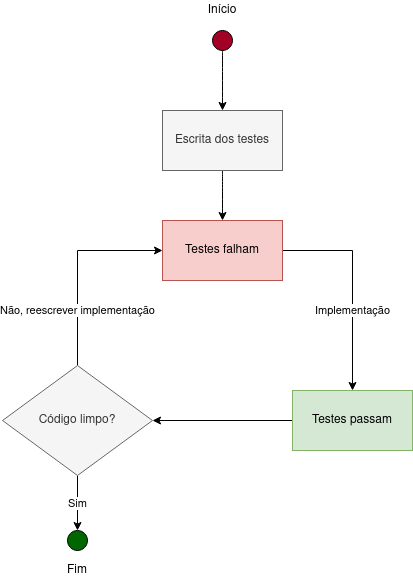
\includegraphics[scale=0.5]{img/tdd.png}
    \caption{Ciclo de desenvolvimento utilizando TDD.}
    \label{fig:tdd-cicle}
\end{figure}

\section{Teste de mutação}

Embora os testes de unidades aplicados no TDD garantam boa cobertura na base de código no sentido de satisfazer especificações de negócio, não há a garantia de que os testes estão garantindo o correto funcionamento do \textit{software}, que é o propósito principal da aplicação de testes. Ou seja, uma boa cobertura de casos de testes não garante que o \textit{software} está sendo testado adequadamente.

O Teste de Mutação de \textit{software} \cite{ieee:mutation-testing-survey} tem como objetivo proporcionar uma melhor avaliação sobre a suíte de casos de teste com base em uma pontuação de adequação. É uma técnica baseada em falhas \cite{ieee:fault-based-testing}, cuja ideia base é gerar alterações no código original, chamados de mutantes, e observar o comportamento dos testes. Por meio da técnica, o código recebe pontuação positiva se o mutante gerado faz com que algum dos testes falhem, no caso da mutação forte, ou com que as saídas sejam alteradas, no caso da mutação fraca. O objetivo principal do teste de mutação é distinguir um programa $P$, o programa correto, de um programa $P'$, o programa incorreto, utilizando-se da hipótese CPH \cite{ieee:hints-on-test-data}, que consiste na premissa de que programadores são competentes e tendem a desenvolver programas próximos do que é correto e as falhas são devidas a pequenas mudanças sintáticas no programa. As mudanças comumente utilizadas no teste de mutação podem ser listadas da forma com que se segue:

\begin{itemize}
    \item Troca de operadores lógicos, como o operador "ou", "e", "not" e "xor"
    \item Troca de operadores comparativos, como igual, diferente, maior, maior ou igual, menor e menor ou igual;
    \item Troca de operadores matemáticos, como mais, menos, produto e divisão; e
    \item Omissão ou troca de chamada de funções ou métodos.
\end{itemize}

\section{Pontos negativos do Teste de Mutação}

O uso do teste de mutação exige que para cada mutação realizada no código fonte original a suíte de casos de testes seja reexecutada novamente, fazendo com que esta técnica seja computacionalmente intensa para grandes bases de código, esse é um dos grandes pontos negativos da técnica de Teste de Mutação. Com isso, a sua aplicação no fluxo do cotidiano do desenvolvedor de \textit{software} fique inviabilizada, fazendo com que ela seja aplicada apenas em projetos cujo custo sobre falhas seja alto o suficiente.


\section{Sistemas de controle de versão de software}

Atualmente o uso de um sistema VCS se tornou algo indispensável para todo desenvolvedor de software \cite{git:review}, são ferramentas auxiliam o desenvolvedor a gerenciar o histórico de mudanças da base de código, juntar trabalhos de vários desenvolvedores, e compartilhar código fonte de forma eficiente. Um desses sistemas mais utilizados na atualidade é o Git \cite{git:website}, que possui também a característica de ser descentralizado, permitindo que o trabalho do desenvolvedor seja feita a qualquer momento, sem a necessidade de conexão com a internet para realizar mudanças na \textit{branch} local.

O fato que torna o uso desses sistemas útil para técnicas de teste de software é o de que se tem o controle de todas partes da base de código estão sendo introduzidas alterações de forma precisa, possibilitando que os testes sejam aplicados aplicados apenas nessas regiões do código fonte original.




\chapter{Trabalhos Anteriores}\label{cap:past-works}

Trabalhos anteriores



\chapter{Proposta}\label{cap:proposal}

Pensando nas dificuldades que o elevado custo computacional associado a utilização da técnica de mutação de software trás, este trabalho se propõe a desenvolver uma técnica para otimizar a aplicação dos testes de mutação por meio do sistema VCM e verificar a efetividade da técnica em um ambiente de desenvolvimento ágil.


\section{Tecnologias associadas}

Para a realização deste trabalho foi escolhida como linguagem de programação o \textit{ECMAScript} \cite{ecma:spec}, conhecido como \textit{Javascript}, por ser a linguagem de programação presente nas principais implementações de navegadores \textit{web} \cite{ecma:mozilla} e ser a mais presente em projetos de \textit{software} de código aberto, segundo uma pesquisa feita na ultima década \cite{ieee:programming-langs}. Para o sistema de versionamento, foi escolhido o Git, por ser comumente utilizado no desenvolvimento de \textit{software} e em projetos de código aberto. Por fim, teve-se como base a biblioteca de mutação de \textit{software} \textit{Stryker Mutator}, por ser amplamente utilizada em \textit{ECMAScript}.

A \cref{tbl:cronograma} apresenta uma estimativa das etapas a serem realizadas durante
o desenvolvimento do trabalho.

\begin{table}[ht]
\centering
\begin{tabular}{c | c}
Etapa do projeto & Período Estimado \\ \hline
\hline
Estudo de implementações da técnica de teste de mutação  & Maio e Junho \\ \\ \hline
Estudo do código fonte do \textit{Stryker Mutator} \\ visando a criação de um \textit{plugin} & Junho \\ \\ \hline
Desenvolvimento de uma POC de \textit{plugin} \\ para o \textit{Stryker Mutator} & Julho \\ \\ \hline
Desenvolvimento de uma POC de \textit{plugin} \\ para o \textit{Stryker Mutator} & Agosto \\ \\ \hline
Medidas de desempenho da aplicação da técnica desenvolvida & Setembro \\ \\ \hline
Análise dos resultados, publicação do código fonte \\ e finalização do trabalho & Outubro \\ \hline
\end{tabular}
\caption{Cronograma de atividades}
\label{tbl:cronograma}
\end{table}




% REFERENCIAS BIBLIOGRAFICAS
\renewcommand\bibname{\itareferencesnamebabel} %renomear título do capítulo referências
\bibliography{referencias}

\annex
\chapter{Exemplo de anexo}\label{anex:wsdl-example}
\begin{minted}{xml}
<?xml version="1.0" encoding="UTF-8"?>
<description xmlns="http://www.w3.org/ns/wsdl"
             xmlns:tns="http://www.tmsws.com/wsdl20sample"
             xmlns:whttp="http://schemas.xmlsoap.org/wsdl/http/"
             xmlns:wsoap="http://schemas.xmlsoap.org/wsdl/soap/"
             targetNamespace="http://www.tmsws.com/wsdl20sample">

<documentation>
  This is a sample WSDL 2.0 document.
</documentation>

<!-- Abstract type -->
  <types>
    <xs:schema xmlns:xs="http://www.w3.org/2001/XMLSchema"
               xmlns="http://www.tmsws.com/wsdl20sample"
               targetNamespace="http://www.example.com/wsdl20sample">

     <xs:element name="request"> ... </xs:element>
     <xs:element name="response"> ... </xs:element>
    </xs:schema>
  </types>

<!-- Abstract interfaces -->
  <interface name="Interface1">
    <fault name="Error1" element="tns:response"/>
    <operation name="Get" pattern="http://www.w3.org/ns/wsdl/in-out">
      <input messageLabel="In" element="tns:request"/>
      <output messageLabel="Out" element="tns:response"/>
    </operation>
  </interface>

<!-- Concrete Binding Over HTTP -->
  <binding name="HttpBinding" interface="tns:Interface1"
           type="http://www.w3.org/ns/wsdl/http">
    <operation ref="tns:Get" whttp:method="GET"/>
  </binding>

<!-- Concrete Binding with SOAP-->
  <binding name="SoapBinding" interface="tns:Interface1"
           type="http://www.w3.org/ns/wsdl/soap"
           wsoap:protocol="http://www.w3.org/2003/05/soap/bindings/HTTP/"
           wsoap:mepDefault="http://www.w3.org/2003/05/soap/mep/request-response">
    <operation ref="tns:Get" />
  </binding>

<!-- Web Service offering endpoints for both bindings-->
  <service name="Service1" interface="tns:Interface1">
    <endpoint name="HttpEndpoint"
              binding="tns:HttpBinding"
              address="http://www.example.com/rest/"/>
    <endpoint name="SoapEndpoint"
              binding="tns:SoapBinding"
              address="http://www.example.com/soap/"/>
  </service>
</description>
\end{minted}



% Glossario
%\itaglossary
%\printglossary

% Folha de Registro do Documento
% Valores dos campos do formulario
\FRDitadata{25 de março de 2015}
\FRDitadocnro{DCTA/ITA/DM-018/2015} %(o número de registro você solicita a biblioteca)
\FRDitaorgaointerno{Instituto Tecnológico de Aeronáutica -- ITA}
%Exemplo no caso de pós-graduação: Instituto Tecnol{\'o}gico de Aeron{\'a}utica -- ITA
\FRDitapalavrasautor{Cupim; Cimento; Estruturas}
\FRDitapalavrasresult{Cupim; Dilema; Construção}
%Exemplo no caso de graduação (TG):
\FRDitapalavraapresentacao{Trabalho de Graduação, ITA, São José dos Campos, 2015. \NumPenultimaPagina\ páginas.}
%Exemplo no caso de pós-graduação (msc, dsc):
%\FRDitapalavraapresentacao{ITA, São José dos Campos. Curso de Mestrado. Programa de Pós-Graduação em Engenharia Aeronáutica e Mecânica. Área de Sistemas Aeroespaciais e Mecatrônica. Orientador: Prof.~Dr. Adalberto Santos Dupont. Coorientadora: Prof$^\textnormal{a}$.~Dr$^\textnormal{a}$. Doralice Serra. Defesa em 05/03/2015. Publicada em 25/03/2015.}
\FRDitaresumo{No contexto do teste de software, uma das principais desvantagens da técnica de Teste de Mutação é o elevado tempo de processamento para a execução das análises em bases de código muito grandes. Este trabalho tem como objetivo desenvolver uma integração com o sistema de versionamento de código fonte Git, de maneira que seja possível realizar testes de mutação rápidos, melhorando a produtividade na utilização dessa técnica no desenvolvimento de software.

Para isso, foi desenvolvido um algoritmo para a aplicação das mutações apenas nas partes do código fonte que estão sendo atualizadas (diffs) para uma nova versão e serão coletadas métricas para avaliar a melhoria no tempo de processamento dos testes. O trabalho será consolidado com a criação de uma biblioteca ou framework para alguma linguagem de programação.

Por fim, este trabalho também se propõe a realizar um estudo sobre a aplicabilidade da técnica desenvolvida no contexto de engenharia de software e desenvolvimento ágil.
}
%  Primeiro Parametro: Nacional ou Internacional -- N/I
%  Segundo parametro: Ostensivo, Reservado, Confidencial ou Secreto -- O/R/C/S
\FRDitaOpcoes{N}{O}
% Cria o formulario
%\itaFRD


\end{document}

% Fim do Documento. O massacre acabou!!! :-)
